%!TEX root = ../template.tex
%%%%%%%%%%%%%%%%%%%%%%%%%%%%%%%%%%%%%%%%%%%%%%%%%%%%%%%%%%%%%%%%%%%%
%% chapter3.tex
%% NOVA thesis document file
%%
%% Chapter with a short latex tutorial and examples
%%%%%%%%%%%%%%%%%%%%%%%%%%%%%%%%%%%%%%%%%%%%%%%%%%%%%%%%%%%%%%%%%%%%

\typeout{NT FILE chapter3.tex}%

\chapter{Work Plan}
\label{cha:work_plan}

Nowadays the cattle in the Coitadinha Farm is separated through physical fences. This solution
leads to great costs and labour expenses, as the fences do not last long and need to be constantly
repaired or replaced. Furthermore, the cows might escape, get lost and potentially get hurt, and the farm
owner might only become aware of this situation when it is too late.
Furthermore to minimize the respective impact on cows on the vegetation, when they remain too
long on the same location, it might useful to change the placement of these fences frequently.

For these reasons we plan to building a collar prototype with the purpose of collecting data,
such as the cows locations and movements, directly from them. This way the farm owners will
receive up to date information about the whereabouts of each cow. We also propose creating a
virtual fence mechanism, where the farm owner can choose the fences locations, as well as
easly change them as required. The virtual fence will keep the cattle inside it through the use of
sound outputs, when a cow starts to get too close to the virtual fence barrier, to try and change
the cows route. If the cow continue to pursue this path the collar will provide a small
frequency electric shock to convence her to go back within the fenced area. This way, the cows will learn that if
they hear the sound output, they should go back, since if they continue they will receive an electric shock.

When studying the animal social behaviours it was recognized that each herds has at least one
leader, which all the other cows in the herd tend to follow. For that reason, we can consider only having
\glsxtrshort{GPS} on these cows, potentially a few more, but not all the cows in the herd. This
way we can reduce overall costs of the system, while still ensuring that we get acurate enough
date with a less need for communication.

Additionally, we need to consider the Coitadinha farm's conditions. It is a vast area with
low cellular coverage which require us to consider solutions to propagate messages, namely
the localization of the virtual fences, from one cow to another until it reaches all of them.
This way it is only needed for one cow to receive this information for it to be propagated in
a decentralized way through the collars of all cows in the herd.
A similar approach must be used to collect the data acquire from each sensor
in the collars worn by the cows back to the end user.

At the end of this work plan, we aim at creating a collar prototype that allows the communication from the user to
the cows and vice-verse to be conducted in a peer-to-peer approach where each cow propagates
the informations from one cow to the next until the information arrives at a mobile base station,
without the need for an infrastructure, in a fully decentralized and ad hoc manner.

\section{Planification}
\label{sec:planification}
The work to be conducted next is divided into separate tasks until its completion,
namely:
\begin{enumerate}
      \item Research
            \begin{enumerate}
                  \item explore the functionalities of three of the existing commercial solutions: the
                        Digital Matter Oyster Edge collar, the Digital Matter Yabby Edge collar and the
                        Nofence collar, mentioned in the Section~\ref{sec:existing_commercial_solutions},
                        and better comprehend how these collars work (we have already started this process
                        to buy these collars).
                  \item  continuously study the way Arduino works during the whole prototype creation
                        process.
            \end{enumerate}
      \item Built Prototype
            \begin{enumerate}
                  \item creation of a rather simple prototype, with help of infrastructures for
                        the communication between nodes and base stations
                  \item explore and create other options for communication, without the need of an
                        infrastructure, leveraging a gossip-based protocol that will be specially tailored
                        for this end.
                  \item development of a virtual fence using sound and/or shocks to maintain the
                        cattle inside it, and a mechanism to change the fence location at the user's
                        desire, using a gossip-based protocol to update the configuration in all collars
                        of a herd.
                  \item augment prototypes applications by adding new sensors to it, possible motion
                        sensors to understand when cows are eating (which is relevant not only to the managers
                        of Herdade da Coitadinha, but also for our partners from FCUL from an ecology research group).
            \end{enumerate}
      \item Testing: testing of final prototype and dense improvements based on test results.
      \item Evaluation: evaluation of the performance of our prototype, using diverse parameters,
            against three previously mentioned commercial solutions.
      \item Completing final report: during the entirety of this work there will be a development
            of the final dissertation report.
\end{enumerate}

Figure~\ref{fig:gantt_charts} provides a Gantt chart planification of the work plan described above.
\begin{figure}[H]
      \caption{Gantt chart of the work plan.}
      \centering
      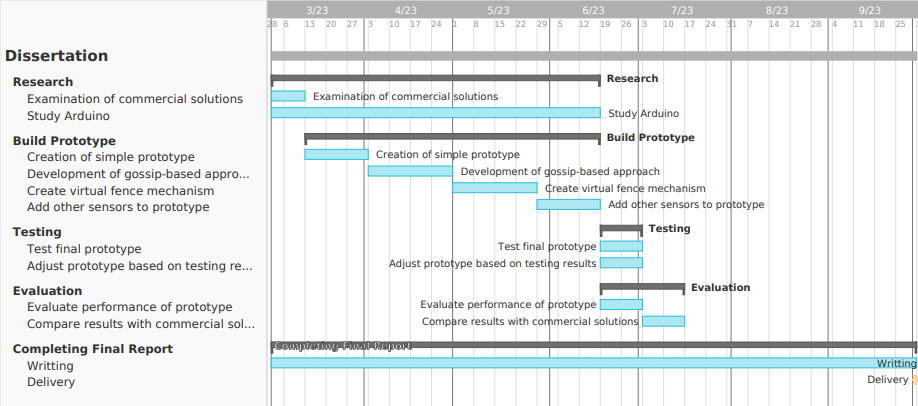
\includegraphics[scale=.8]{Chapters/Figures/gantt_chart.png}
      \label{fig:gantt_charts}
\end{figure}